\documentclass[11pt]{article}
\usepackage{natbib} % our bibliography system 
\usepackage{graphicx} % allows graphics
\usepackage{hyperref} % for adding color and clickable links to references

% configuration of {hyperref} package
\hypersetup{
  colorlinks=true,
  linkcolor=blue,
  citecolor=blue,
  urlcolor=blue
}

\usepackage{amsmath} % allows numbered equations, for one thing
\usepackage{authblk} % to add more authors

\usepackage[a4paper, total={6in, 8in}]{geometry}

\usepackage[dvipsnames]{xcolor} % adds 68 named colors and the ability to define your own, but can cause trouble with beamer and tikz; tikz must be declared after this

\usepackage{mathpazo} % URW Palladio, from Palatino
\usepackage{microtype} % cleans up the kerning and hypenation
\usepackage[margin=15pt,font=small,labelfont={bf}]{caption} % cleans up the structure of the captions

\usepackage{mdframed} % for framed text boxes; does not play well with lineno

% frame style
\mdfdefinestyle{textBox}{%
  linecolor=boxLine,
  outerlinewidth=2pt,
  roundcorner=20pt,
  innertopmargin=-6pt,
  innerbottommargin=10pt,
  innerrightmargin=4pt,
  innerleftmargin=4pt,
  leftmargin = 2pt,
  rightmargin = 2pt,
  backgroundcolor=boxBG
}

\title{Electronic Supplementary Materials for ``Inheritance, Ecology and the Evolution of the Canoes of East Oceania''}
\author[,    1]{Bret A. Beheim\footnote{Corresponding author. babeheim@ucdavis.edu}}
\author[1]{Adrian V. Bell}

\affil[1]{Graduate Group in Ecology, Department of Environmental Science and Policy, University of California, Davis, USA}
\date{26 January 2011}

\begin{document}

\maketitle


\section{Canoe Supplement}

\begin{figure}[h]
\begin{center}
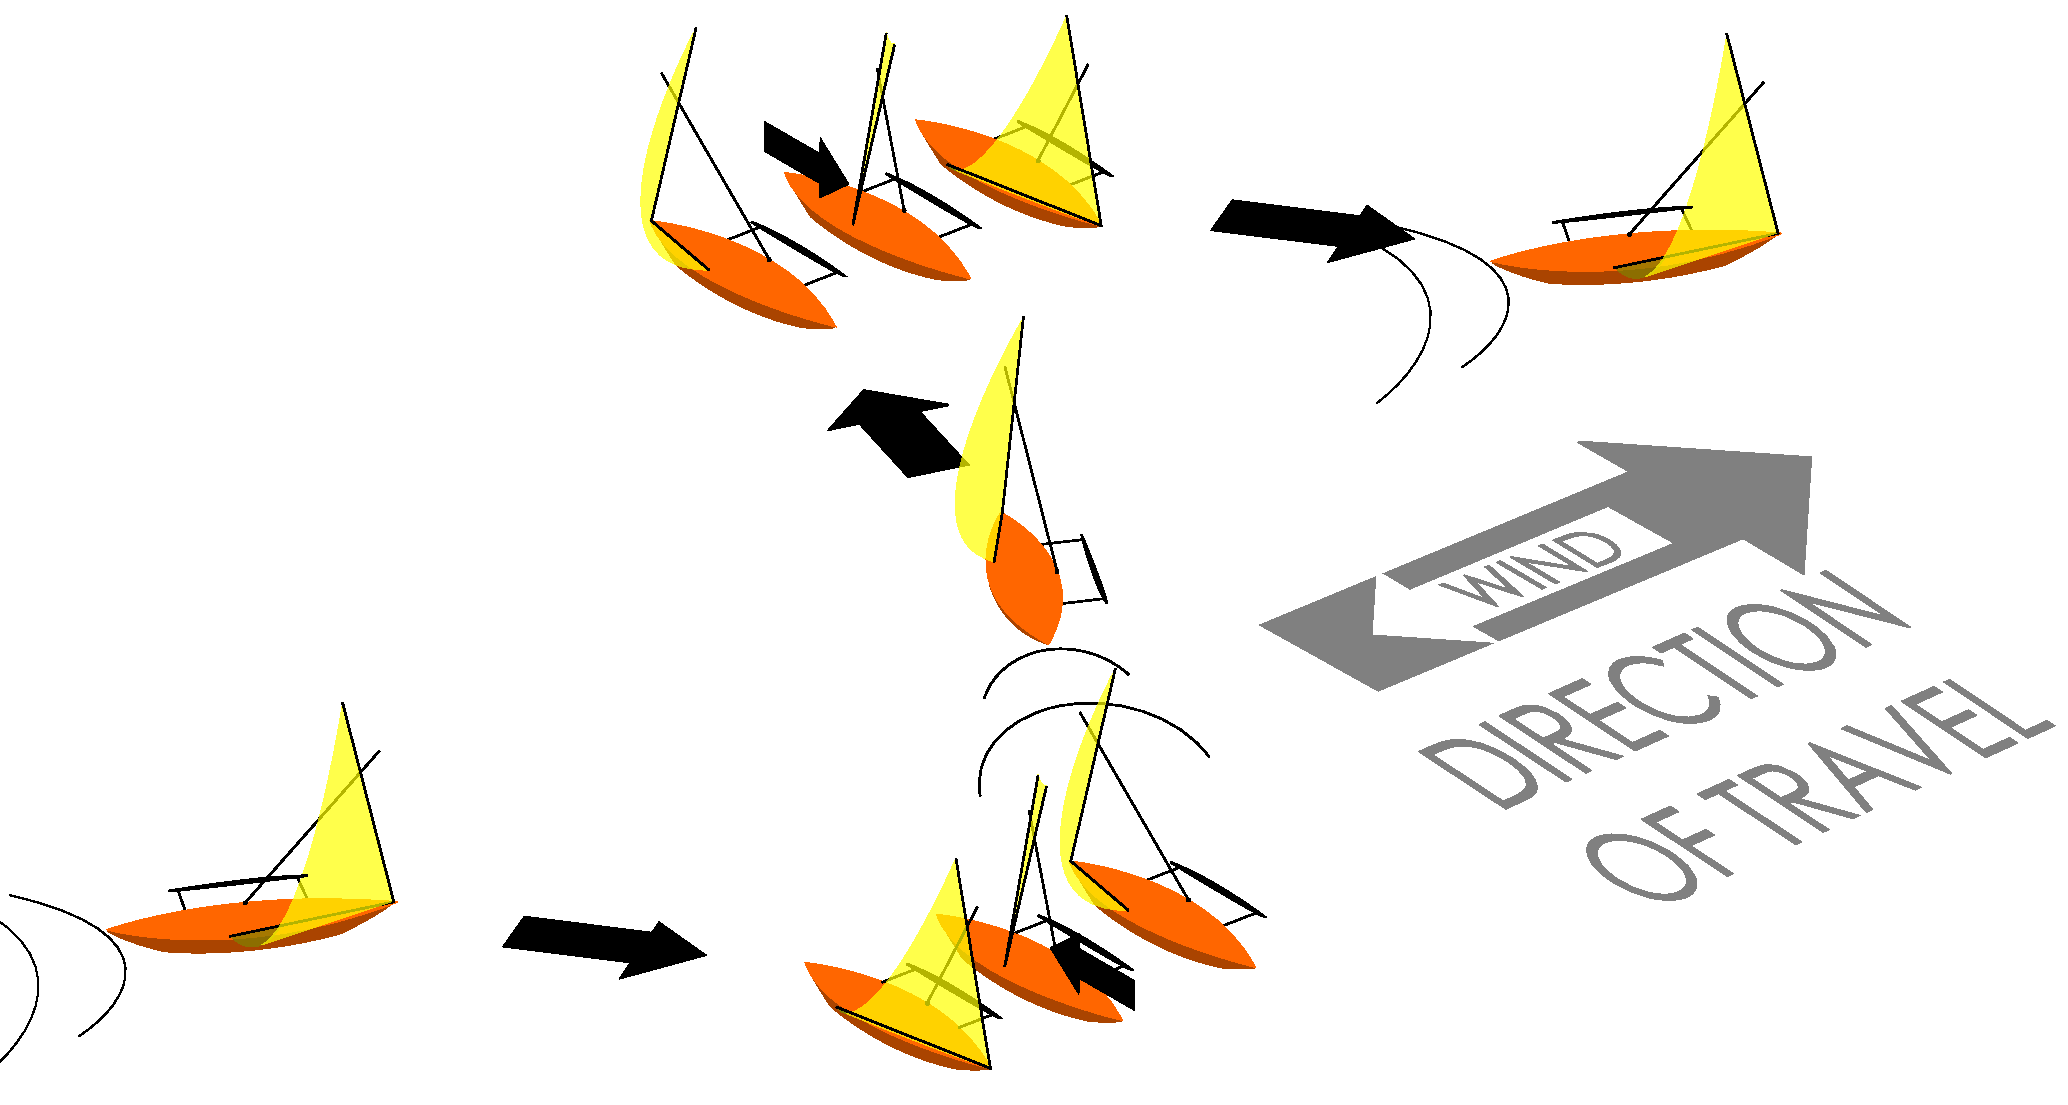
\includegraphics[scale=0.35]{figures/shunting.pdf}
\caption{Illustration of shunting procedure. This technique for moving upwind involves turning the canoe at a right angle from the prevailing wind, manually lifting the tack out of its fore socket, and carefully walking it to the other end of the canoe to insert in an equivalent socket in the aft, reversing the direction of sailing.}
\end{center}
\end{figure}

\begin{figure}[h]
\begin{center}
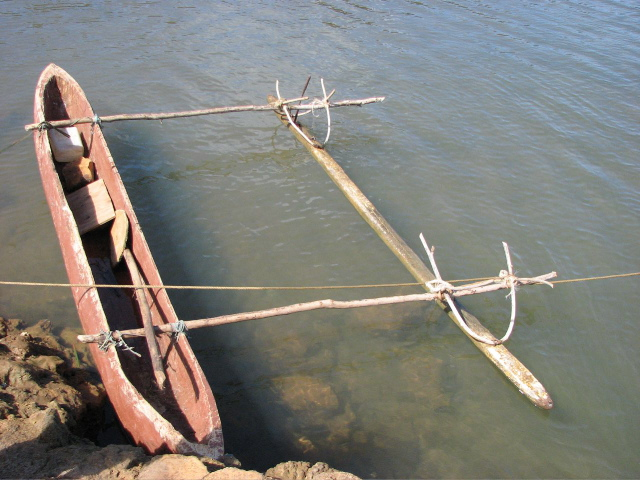
\includegraphics[scale=1.0]{figures/tonganOutrigger.jpg}
\caption{Tongan dugout with outrigger. Two booms and indirect U-shaped stanchions connect main hull to outrigger float. Low freeboard (distance between waterline and gunwale) and lack of washstrakes (added planks along sides to keep the sea out) make this canoe more vulnerable to swamping compared to that in Figure 3. \textit{Photo by A.V. Bell. }}
\end{center}
\end{figure}

\begin{figure}[h]
\begin{center}
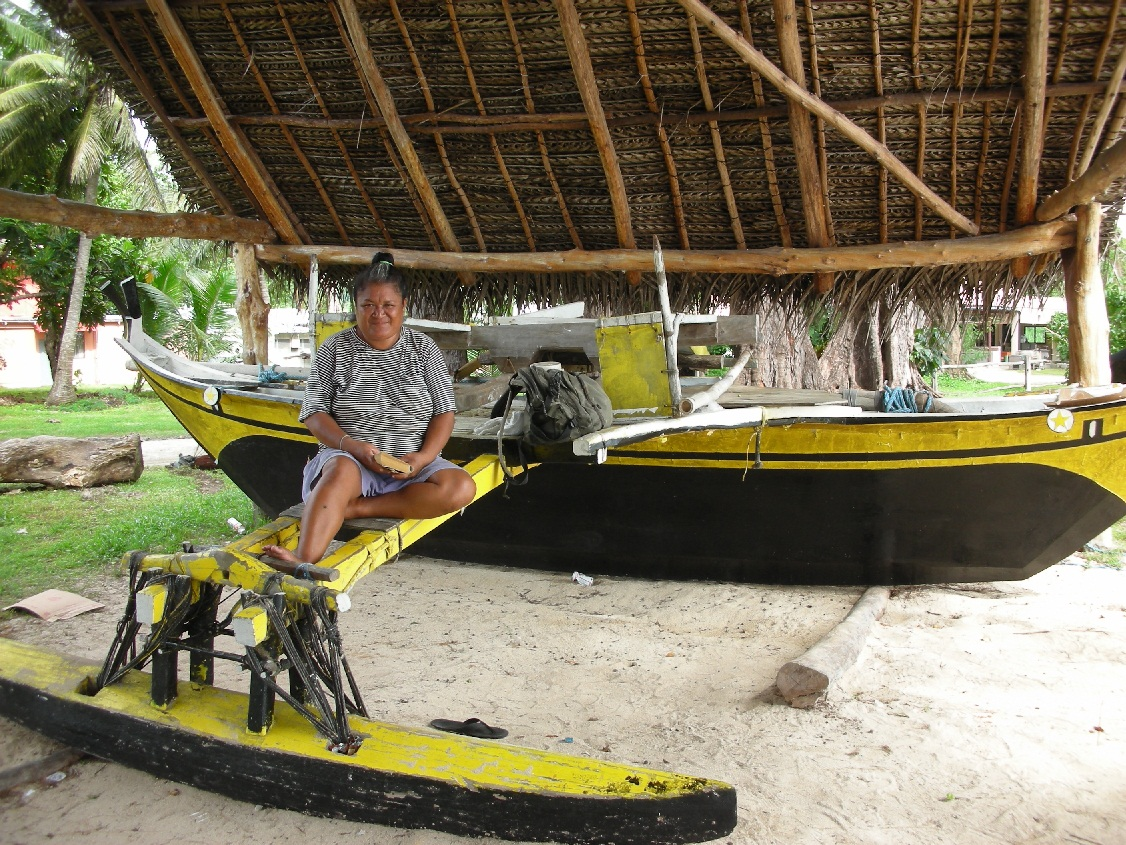
\includegraphics[scale=1]{figures/microOutrigger.jpg}
\caption{Micronesian outrigger. \textit{Photo by Kathryn Demps.}}
\end{center}
\end{figure}

\newpage
\section{Model Selection Methods}

The deviance information criterion is

 \[ DIC = -2 \overline{\log(\mathcal{L}(\widehat{\theta}))} + 2p_D
\]
where $\overline{\log(\mathcal{L}(\widehat{\theta}))}$ is the average deviance over 100,000 simulations using WinBUGS and $p_D$ is the effective number of parameters. The relative distances, rather than absolute magnitudes, of the DIC scores of the models are the basis for comparing them, and so it is common to report each model's $\Delta$ DIC relative to the top model (with the lowest DIC score). Among all R models used in the model comparison, DIC weights are calculating for model $i$ with associated $\Delta$ DIC $d_i$ via

\[w_i = \frac{\exp(-0.5 d_i)}{\sum_{r=1}^R exp(-0.5 d_r)}
\]

Rather than report the parameter estimates from a particular model, we can use the DIC weights and parameter estimates of all models to create model-weighted estimates (Burnham and Anderson, 2002). Specifically, the vector of model-weighted estimates across a set of R models is given by

  \[\widehat{\overline{\theta}} = \sum_{i=1}^R w_i \widehat{\theta}_i
\]
where $\theta_i$ is the estimate of parameter $\theta$ for model $i$, $w_i$ is the DIC weight for model $i$, and $\widehat{\overline{\theta}}$ is the model-averaged estimate of $\theta$. Model-weighted variance is calculated in a similar way, save for an additional term to account for the uncertainty among models (Burnham and Anderson, 2002), yielding
  \[\widehat{var}(\widehat{\overline{\theta}}) = \left[\sum_{i=1}^R w_i \sqrt{\widehat{var}(\widehat{\theta_i}|g_i) + (\widehat{\theta}_i - \widehat{\overline{\theta}})^2}\right]^2
\]

%
%
%-----------------------------------------------
\section{Further Reading}
%-----------------------------------------------
Pacific societies have attracted generations of anthropologists and ecologists for their ability to serve as natural ``laboratories'' of human behavior and socio-ecological processes \citep{Mead1957:PolynesianLab}, and are particularly useful for testing models of cultural transmission and behavioral ecology. Because settlers generally moved west-to-east from the ancestral Lapita homeland in the Bismarks and Solomons, and long-distance voyaging between archipelagos ceased by 1450 CE \citep{Weisler2002:LongVoyagingCollapse}, Pacific island settlements provide an unusually well-partitioned phyletic distribution of cultural variation \citep{KirchGreen2001}. In fact, the isolation of some Polynesian communities has led to cultural divergences that mirror those of the endemic fauna that surround them, allowing anthropologists to use phylogenetic language trees to infer settlement sequences \citep{Gray2000tree, Gray2009:Phylogenies}. On the other hand, it is well understood that ecological conditions played a determining role in the fates of many Pacific societies, and recent Oceanic archaeology has focused on how chemical, biological and climatological gradients both structure and are themselves shaped by agrarian landscapes and socio-political systems \citep{Kirch1984evolution, Kirch2007}.

Within the last fifty years, models of human settlement and dispersion in Fiji and Polynesia have become increasingly ecumenical, supplementing archeology and traditional ethnography \citep{Anderson2006motivation,Feinberg1988seafaring} with structuralist social theory \citep{Sahlins1985:History}, climatology \citep{Anderson2006ENSO}, geochemistry \citep{Collerson2007adze}, genetics \citep{MatisooSmith2004:PacificRatDNA, Whyte2005:PolyHumanEvol, Friedlaender2008:PacificGenetics}, linguistics \citep{Greenhill2005:DispersalTrees}, computational modeling \citep{DiPiazza2007virtualcanoes, Avis2007discovery}, and, in the case of Ben Finney's double-hull \textit{Hokule'a}, experimental seafaring \citep{Finney1994:Rediscovery}. Although the peopling of the Pacific has captured the attention of centuries of scholarship, debates continue about (1) how purposive Polynesian voyaging was \citep{Whyte2005:PolyHumanEvol}, (2) the sequence and methods of settlement \citep{Irwin1992}, (3) how quickly it occurred \citep{Anderson2000:Slowboats, Thomas2008:Lastpulse, Gray2009:Phylogenies}, (4) the extent of pre-European trade and interaction  \citep{Weisler1998}, (5) the kinds of canoes and sailing rigs employed in these processes \citep{Doran1981canoes, Anderson2001:SharpEnd}, and (6) the evolutionary pressures that shaped them \citep{Horridge1987:IndonesiaCanoes}.

%-----------------------------------------------
\section{Data Reprocessing}
%-----------------------------------------------

Our dataset classified 65 distinct canoe traits based on descriptions in \cite{HaddonHornell1936}'s \textit{Canoes of Oceania}. Beginning with \cite{rogers2008:Canoes}'s 134-trait dataset, we excluded or merged traits which were most likely to be affected by recording biases, practical dependencies and coding errors.

For example, although encyclopedic in their treatment, \cite{HaddonHornell1936} employ an inconsistent use of certain terms, such as \textit{sennit} and \textit{coir}, whose distinctiveness is critical to traits coded as OAH12, OAH13 and DAH11. In such cases, traits were merged to eliminate the potential for artificial distinction. 

Additionally, since many of the descriptions in \textit{Canoes of Oceania} were culled by Haddon \& Hornell from a hodgepodge of accounts by European explorers, missionaries, merchants, and scholars over a period of several hundred years, the potential for simple omission of a canoe trait actually present on an island group is considerable. That Fijian double canoes ranged from 25 to 72 feet in length, 97 to 120 feet in length, but not in-between suggests the presence of a ethnographic sampling bias, rather than some actual design preference or constraint. 

In some cases, the supplementary table in \cite{rogers2008:Canoes} is clearly missing data; use of Hawaiian canoes for fishing was coded as ``absent'' (OCP2, DCP2), even though both double-hull and outrigger canoes had fishing-pole rests (OAF1, DAF1). Similarly, though outrigger canoes were common in both the Australs and Tonga, traits OAO1 (``Outrigger present on port side'') and OAO2 (``Outrigger present on starboard side'') are both coded as ``absent'' for these archipelagos, a logical impossibility. Coding the orientation of the outrigger floats is particularly problematic because Polynesian canoes were often designed to sail with either end facing forward and have no permanent starboard and port, rendering such traits essentially meaningless. To circumvent this problem, we excluded traits likely to be missing data points or whose presence in the island group was ambiguous among the primary sources.

Furthermore, several traits were excluded because of likely influence of practical interdependencies, invisible to covariance screening tests because of potentially large sampling biases and the confused nomenclature in \textit{Canoes of Oceania}. For example, ``mast stepped forward'' and ``Oceanic Lateen sail present'' are treated in the original dataset as independent traits, despite the fact that the former is a necessary component of the latter \citep{Doran1981canoes}. Doran's survey of Austronesian canoe designs synthesizes a variety of reports by \cite{HaddonHornell1936} into distributional maps, and also provides the basis for our data on the distribution of shunting and the use of the primitive crane sprit.     

Finally, we compacted equivalent double-hull traits and outrigger traits, on the premise that any discrepancies between the two categories represent noise rather than useful information. Considering the regularity by which outrigger and double-hulled canoes were converted from one to the other in Polynesia, the notion that traits on one canoe type should be distinct from traits on the other does not appear tenable.


\section{Model Specification and Estimation}

We introduce some notation to describe trait distributions and our models. Let $i \in \{1,2, \dots ,11\}$ index island group and $t \in \{1,2,\dots,65\}$ index canoe traits. Then binary variable $x_{t,i} \in \{0,1\}$ describes the presence or absence of trait $t$ on island group $i$ for the 65 $\times$ 11 matrix of island traits $X$.

Using the currently understood colonization sequence (see Figure 1 of the main text), let $C_i$ be the set of island groups within the region that colonized island group $i$, and $|C_i|$ be the number of island groups in $C_i$. Now, the frequency of trait $t$ in the colonizing region $C_i$ of island group $i$ is $y_{t,i} = \left( \sum_{j \in C_i} x_{t,j} \right) / |C_i|$. Now let $S_i$ be the set of island groups within the sphere of influence of island group $i$, based on the zones of interaction compiled by Weisler (1998), and $|S_i|$ be the number of island groups in $S_i$. Then the frequency of trait $t$ in the sphere of influence $S_i$ of island group $i$ is $m_{t,i}= \left(\sum_{j \in S_i} x_{t,j} \right) / |S_i|$. Because data sources are not properly collected statistical samples in any sense, we should consider that the presence of a trait in a region is more diagnostic for cultural transmission than its observed frequency (as recorded in \cite{HaddonHornell1936}). Hence, for interaction spheres, we also consider sphere presence/absence models using $p_{t,i}= 1$ if $m_{t,i}>0$, and $0$ otherwise.

Since the goal is to predict $x_{t,i} \in \{0,1\}$, the general form of the model for trait $t$ is
    \[\mathrm{Logit} \Pr( x_{t,i}=1 ) = \alpha_t + B Z_i \],
where $Z_i$ is a vector of ecological and cultural inheritance covariates for island $i$ and $B$ is a vector of coefficients. Table~\ref{tab:models} shows examples of null (N) models, cultural inheritance (C) models, ecological (E)  models, and the cultural inheritance-ecological (CE) models.

Using a Gibbs sampler implemented in the software \texttt{R} and \texttt{Winbugs}, we estimate posterior distributions and the Deviance Information Criterion (DIC). For each run of the Gibbs sampler we perform 100,000 interations with a burn-in of 50,000 interations. Starting values for continuous parameters were randomly drawn from a Gaussian distribution with mean zero and variance 1, and binary parameters randomly drawn from a Binomial distribution with the probability of a success (drawing a value of one) equal to one-half.

\begin{table}[t]
\begin{center}
\begin{footnotesize}
\begin{tabular}{p{7.5cm} p{7cm}}
\bf{Model name} & $ \text{Logit }Pr(x_{t,i}=1) =$\\
\hline
{\em Null models}& \\
\hline
N1: Weighted coinflip & $ \alpha $ \\
N2: Base & $ \alpha_t $ \\
\hline
{\em Inheritance} & \\
\hline
C1: Past & $\alpha_t + \beta_1 y_{t,i}$ \\
C2: Past \& Sphere Present & $\alpha_t + \beta_1 y_{t,i} + \beta_2 p_{t,i} $ \\
\hline
{\em Ecology} & \\
\hline
E1: Island area &  $\alpha_t + \beta a_i$ \\
E2: Reef high \& low \& Atoll & $\alpha_t + \kappa_1 r_{h,i} + \kappa_2 r_{l,i} + \kappa_3 r_{a,i}$ \\
\hline
{\em Inheritance \& Ecology} & \\
\hline
CE1: Past \& Area & $\alpha_t + \gamma y_{t,i} + \beta a_i$ \\
CE6: Past \& Sphere Present \& Area \& Island type & $\alpha_t + \gamma y_{t,i} + \lambda p_{t,i} + \beta a_i + \kappa_1 r_{h,i} + \kappa_2 r_{l,i} + \kappa_3 r_{a,i}$ \\
\hline
\end{tabular}
\end{footnotesize}
\end{center}
\caption{Representative models of those considered in this analysis. The average island size in the focal archipelago ($a_i$), and ``Island Type'' represents ``Reef high'' ($r_{h,i}$), ``Reef low'' ($r_{l,i}$), or ``Atoll'' ($r_{a,i}$).}
\label{tab:models}
\end{table}

\clearpage
\fbox{
\parbox{6in}{Box 1. Description of Bayesian Statistical terms used in the text \\
\textbf{Bayesian statistics:} A branch of statistics that focuses on estimating the probability density function of unknown parameters using a prior distribution, the observations, and Bayes' theorem. In this way, assertions about unknown parameters are not expressed by attempting to cover true values with confidence intervals; instead, the emphasis is on making probabilistic statements using distributions \citep{Gill2008}.\\
\textbf{Credible intervals:} The 100$(1-a)$\% credible interval gives the region of the parameter space in which the probability of covering parameters $\Theta$ is equal to $(1-a)$. Unlike the frequentist confidence interval, there is no presumption of a true parameter value to estimate. 
We report 95\% credible intervals in Table \ref{tab:modelComparisonsDecorative}. \citep{Gill2008}.\\
\textbf{Deviance Information Criteria (DIC):} A value used to compare model performance with other competing models. The relative value compared to other models, not the actual number, is used to compare the performance of the model. It is a Bayesian analog to Akaike Information Criteria (AIC) which is more commonly known in model selection. \\
\textbf{Gibbs sampler:} A sampling algorithm that is an example of Markov Chain Monte Carlo methods used to estimate an integral that cannot be solved analytically. Most posterior distributions cannot be solved analytically, therefore this and similar methods are essential for parameter estimation. \\
\textbf{Posterior distribution:} A probability density function of posterior probabilities used to estimate the unknown parameters and their credible intervals. Posterior probabilities are conditional probabilities with the Bayesian prior, the likelihood, and a normalizing constant as key components. Most often these can only be estimated using Markov Chain Monte Carlo methods. \\
\textbf{Markov Chain Monte Carlo:} Because the posterior density function for unknown parameters usually cannot be solved analytically, this stochastic numerical method is used to provide an estimate of the posterior distribution.\\
\textbf{Bayesian priors:} also known as prior density functions, are propositions or statements concerning the values of unknown parameters before estimation. These are expressed as probability density functions such as the Normal (Gaussian) distribution, or commonly the Beta distribution. The prior and the likelihood of the data given a model are key components of the posterior distribution. \\
}
}

\begin{table}
\begin{center}
\begin{tabular}{lllll}
Models & DIC & $\Delta$ DIC & $w$\\
\hline
mPast2ReefHighLowAtoll & 944.75 & 0 & 0.67\\
mPast2AreaReefHighLowAtoll & 946.56 & 1.81 & 0.27\\
mPast2SpherePresentAreaReefHighLowAtoll & 950.43 & 5.68 & 0.04\\
mPast2Area & 953.01 & 8.26 & 0.01\\
mReefHighLowAtoll & 954.64 & 9.89 & $<$0.01\\
mReefHighAtoll & 955.35 & 10.6 & $<$0.01\\
mPast2SphereMeanAreaReefHighLowAtoll & 956.23 & 11.48 & $<$0.01\\
\textbf{mBase} & \textbf{957.57} & \textbf{12.82} & \textbf{$<$0.01}\\
mPast2SphereMeanArea & 958.33 & 13.58 & $<$0.01\\
mPast2 & 958.46 & 13.71 & $<$0.01\\
mArea & 959.5 & 14.75 & $<$0.01\\
mSphereMean & 959.78 & 15.03 & $<$0.01\\
mSpherePresent & 960.57 & 15.82 & $<$0.01\\
mAreaReefHighAtoll & 960.81 & 16.06 & $<$0.01\\
mAreaReefHighLowAtoll & 963.3 & 18.55 & $<$0.01\\
mPast2SpherePresentArea & 965.16 & 20.41 & $<$0.01\\
mPastReefHighLowAtoll & 969.62 & 24.87 & $<$0.01\\
mPastSphereMeanAreaReefHighLowAtoll & 971.35 & 26.6 & $<$0.01\\
mPastSpherePresentAreaReefHighLowAtoll & 978.44 & 33.69 & $<$0.01\\
mPastAreaReefHighLowAtoll & 981.08 & 36.33 & $<$0.01\\
mCoinFlip & 989.51 & 44.76 & $<$0.01\\
mPastSphereMeanArea & 1022.93 & 78.18 & $<$0.01\\
mPastSpherePresent & 1027.01 & 82.26 & $<$0.01\\
mPastSpherePresentArea & 1033.41 & 88.66 & $<$0.01\\
mPastSphereMean & 1037.35 & 92.6 & $<$0.01\\
mPastArea & 1047.06 & 102.31 & $<$0.01\\
mPast & 1048.18 & 103.43 & $<$0.01\\
\end{tabular}
\end{center}
\caption{Model rankings for all canoe traits. $\Delta$ DIC is the difference between a model's DIC score and the top model's, and DIC weights ($w$) quantify the relative performance among models. The best-performing null model is highlighted in bold; models with higher rankings (lower DIC scores) are plausibly better at explaining the data than the null model.}
\label{tab:modelComparisonsAllTraits}
\end{table}

\begin{table}
\begin{center}
\begin{tabular}{lllll}
Models & DIC & $\Delta$ DIC & $w$\\
\hline
mSpherePresent & 55.69 & 0.00 & 0.13\\
mPastSpherePresent & 56.11 & 0.42 & 0.11\\
\textbf{mBase} & \textbf{56.98} & \textbf{1.29} & \textbf{0.07}\\
mReefHighAtoll & 57.17 & 1.48 & 0.06\\
mArea & 57.25 & 1.56 & 0.06\\
mPastArea & 57.63 & 1.94 & 0.05\\
mPast & 57.71 & 2.02 & 0.05\\
mPastSpherePresentArea & 57.73 & 2.04 & 0.05\\
mSphereMean & 57.87 & 2.18 & 0.04\\
mPast2Area & 57.93 & 2.24 & 0.04\\
mPastSphereMean & 58.25 & 2.56 & 0.04\\
mAreaReefHighAtoll & 58.35 & 2.66 & 0.03\\
mPast2SpherePresentArea & 58.39 & 2.69 & 0.03\\
mPast2 & 58.41 & 2.72 & 0.03\\
mPastSpherePresentAreaReefHighLowAtoll & 58.80 & 3.11 & 0.03\\
mReefHighLowAtoll & 58.90 & 3.20 & 0.03\\
mPastSphereMeanArea & 59.19 & 3.50 & 0.02\\
mPast2ReefHighLowAtoll & 59.31 & 3.62 & 0.02\\
mPast2SphereMeanArea & 59.68 & 3.99 & 0.02\\
mPastReefHighLowAtoll & 59.81 & 4.12 & 0.02\\
mAreaReefHighLowAtoll & 59.97 & 4.28 & 0.02\\
mPastAreaReefHighLowAtoll & 60.70 & 5.01 & 0.01\\
mPast2AreaReefHighLowAtoll & 60.94 & 5.25 & 0.01\\
mPast2SpherePresentAreaReefHighLowAtoll & 61.40 & 5.71 & 0.01\\
mPastSphereMeanAreaReefHighLowAtoll & 61.65 & 5.96 & 0.01\\
mCoinFlip & 62.08 & 6.39 & 0.01\\
mPast2SphereMeanAreaReefHighLowAtoll & 63.06 & 7.37 & $<$0.01\\
\end{tabular}
\end{center}
\caption{Model rankings for decorative canoe traits.}
\label{tab:modelComparisonsDecorative}
\end{table}

\begin{table}
\begin{center}
\begin{tabular}{lllll}
Models & DIC & $\Delta$ DIC & $w$\\
\hline
mPastSphereMean & 115.62 & 0.00 & 0.11\\
mSpherePresent & 115.62 & 0.00 & 0.11\\
mPast & 115.89 & 0.27 & 0.10\\
mPastSpherePresent & 116.16 & 0.54 & 0.09\\
mPastArea & 116.34 & 0.72 & 0.08\\
mPast2 & 116.58 & 0.96 & 0.07\\
mPastSpherePresentArea & 117.37 & 1.75 & 0.05\\
mAreaReefHighAtoll & 117.37 & 1.75 & 0.05\\
mPast2Area & 117.51 & 1.89 & 0.04\\
mReefHighAtoll & 117.64 & 2.02 & 0.04\\
mPastReefHighLowAtoll & 118.00 & 2.38 & 0.03\\
mPast2SpherePresentArea & 118.10 & 2.49 & 0.03\\
mPastSphereMeanArea & 118.40 & 2.78 & 0.03\\
mSphereMean & 118.79 & 3.17 & 0.02\\
\textbf{mBase} & \textbf{118.90} & \textbf{3.28} & \textbf{0.02}\\
mPast2SphereMeanArea & 119.09 & 3.47 & 0.02\\
mArea & 119.12 & 3.50 & 0.02\\
mAreaReefHighLowAtoll & 119.40 & 3.78 & 0.02\\
mReefHighLowAtoll & 119.92 & 4.30 & 0.01\\
mPast2ReefHighLowAtoll & 119.94 & 4.32 & 0.01\\
mPast2AreaReefHighLowAtoll & 120.29 & 4.67 & 0.01\\
mPast2SpherePresentAreaReefHighLowAtoll & 120.45 & 4.84 & 0.01\\
mPastSpherePresentAreaReefHighLowAtoll & 121.10 & 5.48 & 0.01\\
mPastSphereMeanAreaReefHighLowAtoll & 121.28 & 5.66 & 0.01\\
mPastAreaReefHighLowAtoll & 122.00 & 6.38 & $<$0.01\\
mPast2SphereMeanAreaReefHighLowAtoll & 122.70 & 7.08 & $<$0.01\\
mCoinFlip & 123.30 & 7.68 & $<$0.01\\
\end{tabular}
\end{center}
\caption{Model rankings for double-hull canoe traits.}
\label{tab:modelComparisonsDouble}
\end{table}

\begin{table}
\begin{center}
\begin{tabular}{lllll}
Models & DIC & $\Delta$ DIC & $w$\\
\hline
mPastAreaReefHighLowAtoll & 269.13 & 0.00 & 0.41\\
mPastSphereMeanArea & 270.84 & 1.70 & 0.18\\
mPastSphereMeanAreaReefHighLowAtoll & 271.47 & 2.34 & 0.13\\
mPastSpherePresentAreaReefHighLowAtoll & 273.32 & 4.19 & 0.05\\
mPastSphereMean & 273.86 & 4.72 & 0.04\\
mPastReefHighLowAtoll & 274.13 & 4.99 & 0.03\\
mPastArea & 274.52 & 5.39 & 0.03\\
mPast2Area & 274.87 & 5.73 & 0.02\\
mPast2SphereMeanArea & 275.09 & 5.95 & 0.02\\
mPast2 & 275.26 & 6.12 & 0.02\\
mPast2SpherePresentArea & 276.52 & 7.38 & 0.01\\
\textbf{mBase} & \textbf{276.95} & \textbf{7.82} & \textbf{0.01}\\
mPast2ReefHighLowAtoll & 277.11 & 7.98 & 0.01\\
mArea & 277.37 & 8.23 & 0.01\\
mPast2AreaReefHighLowAtoll & 277.50 & 8.37 & 0.01\\
mPastSpherePresentArea & 278.12 & 8.99 & $<$0.01\\
mSphereMean & 278.16 & 9.02 & $<$0.01\\
mSpherePresent & 278.90 & 9.77 & $<$0.01\\
mPastSpherePresent & 279.27 & 10.14 & $<$0.01\\
mPast2SpherePresentAreaReefHighLowAtoll & 279.86 & 10.73 & $<$0.01\\
mPast & 280.17 & 11.04 & $<$0.01\\
mReefHighAtoll & 280.22 & 11.08 & $<$0.01\\
mPast2SphereMeanAreaReefHighLowAtoll & 280.32 & 11.19 & $<$0.01\\
mAreaReefHighAtoll & 280.89 & 11.76 & $<$0.01\\
mReefHighLowAtoll & 281.34 & 12.21 & $<$0.01\\
mAreaReefHighLowAtoll & 282.17 & 13.04 & $<$0.01\\
mCoinFlip & 284.42 & 15.28 & $<$0.01\\
\end{tabular}
\end{center}
\caption{Model rankings for hull traits.}
\label{tab:modelComparisonsHull}
\end{table}

\begin{table}
\begin{center}
\begin{tabular}{lllll}
Models & DIC & $\Delta$ DIC & $w$\\
\hline
mPast2ReefHighLowAtoll & 232.36 & 0.00 & 0.42\\
mPast2SphereMeanAreaReefHighLowAtoll & 233.33 & 0.98 & 0.26\\
mReefHighLowAtoll & 236.03 & 3.67 & 0.07\\
mAreaReefHighLowAtoll & 236.35 & 3.99 & 0.06\\
mPast2AreaReefHighLowAtoll & 236.86 & 4.50 & 0.04\\
mPast2SpherePresentAreaReefHighLowAtoll & 237.61 & 5.26 & 0.03\\
mPastSpherePresentArea & 238.24 & 5.88 & 0.02\\
mPastSphereMeanAreaReefHighLowAtoll & 239.11 & 6.76 & 0.01\\
mPast2SphereMeanArea & 239.79 & 7.43 & 0.01\\
mSphereMean & 240.07 & 7.71 & 0.01\\
mPastSphereMeanArea & 240.07 & 7.72 & 0.01\\
mPast2 & 240.09 & 7.73 & 0.01\\
\textbf{mBase} & \textbf{240.15} & \textbf{7.79} & \textbf{0.01}\\
mReefHighAtoll & 240.26 & 7.90 & 0.01\\
mAreaReefHighAtoll & 240.53 & 8.18 & 0.01\\
mPast2SpherePresentArea & 241.20 & 8.84 & 0.01\\
mArea & 241.28 & 8.93 & $<$0.01\\
mSpherePresent & 241.88 & 9.53 & $<$0.01\\
mPastReefHighLowAtoll & 243.08 & 10.72 & $<$0.01\\
mPast2Area & 244.03 & 11.68 & $<$0.01\\
mPastArea & 244.84 & 12.48 & $<$0.01\\
mPastSpherePresentAreaReefHighLowAtoll & 245.01 & 12.65 & $<$0.01\\
mPastAreaReefHighLowAtoll & 245.28 & 12.93 & $<$0.01\\
mCoinFlip & 245.81 & 13.45 & $<$0.01\\
mPastSphereMean & 246.74 & 14.38 & $<$0.01\\
mPast & 248.77 & 16.41 & $<$0.01\\
mPastSpherePresent & 249.22 & 16.87 & $<$0.01\\
\end{tabular}
\end{center}
\caption{Model rankings for outrigger canoe traits.}
\label{tab:modelComparisonsOutrigger}
\end{table}

\begin{table}
\begin{center}
\begin{tabular}{lllll}
Models & DIC & $\Delta$ DIC & $w$\\
\hline
mPastSphereMean & 123.91 & 0.00 & 0.32\\
mPast2SphereMeanArea & 126.26 & 2.35 & 0.10\\
mPastSphereMeanArea & 126.64 & 2.73 & 0.08\\
mPastSpherePresentArea & 126.90 & 2.99 & 0.07\\
mPastSphereMeanAreaReefHighLowAtoll & 127.20 & 3.29 & 0.06\\
mPast & 127.59 & 3.68 & 0.05\\
mPastSpherePresent & 127.98 & 4.07 & 0.04\\
mSphereMean & 128.37 & 4.45 & 0.03\\
mPastArea & 128.60 & 4.69 & 0.03\\
mArea & 129.01 & 5.09 & 0.03\\
mPast2SpherePresentArea & 129.03 & 5.12 & 0.02\\
\textbf{mBase} & \textbf{129.18} & \textbf{5.27} & \textbf{0.02}\\
mPast2SphereMeanAreaReefHighLowAtoll & 129.20 & 5.28 & 0.02\\
mPast2 & 129.53 & 5.61 & 0.02\\
mPast2Area & 129.67 & 5.76 & 0.02\\
mPastSpherePresentAreaReefHighLowAtoll & 130.96 & 7.05 & 0.01\\
mReefHighAtoll & 131.00 & 7.09 & 0.01\\
mReefHighLowAtoll & 131.16 & 7.25 & 0.01\\
mSpherePresent & 131.32 & 7.41 & 0.01\\
mAreaReefHighAtoll & 131.49 & 7.58 & 0.01\\
mPast2SpherePresentAreaReefHighLowAtoll & 131.79 & 7.88 & 0.01\\
mPastAreaReefHighLowAtoll & 131.81 & 7.89 & 0.01\\
mAreaReefHighLowAtoll & 131.93 & 8.02 & 0.01\\
mPastReefHighLowAtoll & 132.17 & 8.26 & 0.01\\
mPast2ReefHighLowAtoll & 132.57 & 8.66 & 0.00\\
mPast2AreaReefHighLowAtoll & 133.86 & 9.95 & 0.00\\
mCoinFlip & 135.62 & 11.71 & 0.00\\
\end{tabular}
\end{center}
\caption{Model rankings for all paddle traits.}
\label{tab:modelComparisonsPaddle}
\end{table}

\begin{table}
\begin{center}
\begin{tabular}{lllll}
Models & DIC & $\Delta$ DIC & $w$\\
\hline
mPastAreaReefHighLowAtoll & 132.27 & 0.00 & 0.18\\
mPastArea & 132.31 & 0.04 & 0.18\\
mPastSphereMeanArea & 133.16 & 0.89 & 0.11\\
mPastSpherePresentArea & 133.40 & 1.13 & 0.10\\
mPast2 & 134.39 & 2.12 & 0.06\\
mPast & 134.49 & 2.22 & 0.06\\
mPast2Area & 135.10 & 2.83 & 0.04\\
mPastSpherePresentAreaReefHighLowAtoll & 135.53 & 3.26 & 0.04\\
mPast2SpherePresentArea & 135.71 & 3.44 & 0.03\\
mPast2SphereMeanArea & 135.74 & 3.47 & 0.03\\
mPastSphereMean & 135.77 & 3.50 & 0.03\\
mPastSpherePresent & 136.56 & 4.29 & 0.02\\
\textbf{mBase} & \textbf{136.66} & \textbf{4.38} & \textbf{0.02}\\
mPastSphereMeanAreaReefHighLowAtoll & 136.79 & 4.52 & 0.02\\
mArea & 136.94 & 4.66 & 0.02\\
mSphereMean & 137.94 & 5.67 & 0.01\\
mReefHighAtoll & 138.80 & 6.53 & 0.01\\
mPast2AreaReefHighLowAtoll & 138.81 & 6.53 & 0.01\\
mPastReefHighLowAtoll & 138.82 & 6.55 & 0.01\\
mSpherePresent & 138.97 & 6.70 & 0.01\\
mCoinFlip & 139.31 & 7.03 & 0.01\\
mPast2ReefHighLowAtoll & 139.81 & 7.54 & $<$0.01\\
mAreaReefHighAtoll & 140.05 & 7.77 & $<$0.01\\
mPast2SphereMeanAreaReefHighLowAtoll & 141.02 & 8.75 & $<$0.01\\
mAreaReefHighLowAtoll & 141.29 & 9.02 & $<$0.01\\
mReefHighLowAtoll & 141.30 & 9.03 & $<$0.01\\
mPast2SpherePresentAreaReefHighLowAtoll & 142.46 & 10.18 & $<$0.01\\
\end{tabular}
\end{center}
\caption{Model rankings for sail and rigging traits.}
\label{tab:modelComparisonsSailRigging}
\end{table}

\newpage

\bibliographystyle{plainnat} % bibtex requires a style
\bibliography{references} % pointing to references.bib

\end{document}








